%% Journal of Open Research Software Latex template -- Created By Stephen Bonner and John Brennan, Durham Universtiy, UK.

\documentclass{jors}

%% Set the header information
\pagestyle{fancy}
\definecolor{mygray}{gray}{0.6}
\renewcommand\headrule{}
\rhead{\footnotesize 3}
\rhead{\textcolor{gray}{UP JORS software Latex paper template version 0.1}}


\usepackage{amsthm,amsmath}
\usepackage{graphicx}
\usepackage{listings,url}

\lstset{language=Python}
% additional python keywords
\lstset{
    morekeywords={with, as}
}
 %additional package kewords
%\lstset{
    %morekeywords={Pymrio, country_converter, coco, matplotlib, pyplot, plt, seaborn, sns}
%}

% additional method keywords
%\lstset{
 %morekeywords={parse_wiod, download_wiod2013, get_sectors, get_regions, diag_stressor,
               %calc_x, calc_A, calc_all, agg_conc, country_converter, aggregate, rename_regions,
               %style, context, savefig, show, plot_account, groupby}
%}


\begin{document}

{\bf Software paper for submission to the Journal of Open Research Software} 
Please submit the completed paper to: editor.jors@ubiquitypress.com

\rule{\textwidth}{1pt}

\section*{(1) Overview}

\vspace{0.5cm}

\section*{Title}

Pymrio - a Python based Multi-Regional Input-Output Analysis toolbox

\section*{Paper Authors}

{1. Stadler, Konstantin

\section*{Paper Author Roles and Affiliations}
Developer of Pymrio, Industrial Ecology Programme, Norwegian University of Science and Technology (NTNU)

\section*{Abstract}

Pymrio is an open source tool for Environmentally Extended Multi-Regional Input-Output (EE MRIO) analysis developed in Python.
It provides a high-level abstraction layer for global EE MRIO databases in order to simplify common EE MRIO data tasks. 
Among others, Pymrio includes parsers for several openly available EE MRIO databases (EXIOBASE v1 - v3, WIOD, Eora26) as well as methods for production and consumption based accounts calculation, aggregation, stressor origin estimation and visualization. 
The use of a consistent storage format including meta data and modification history for MRIOs allows to exchange data with other analysis tools, aiming for an increased interoperability of Industrial Ecology analysis software.

\section*{Keywords}

Sustainability Analysis; Multi Regional Input Output Analysis; Footprinting, Consumption Based Accounting, EXIOBASE, WIOD, Eora26, Python

\section*{Introduction}

Environmentally Extended Multi-Regional Input-Output (EE MRIO) tables describe economic relationships within and between regions and their environmental repercussions. The analysis of the these tables has become the prevailing methodology in Industrial Ecology and sustainability science to evaluate globally spanning supply chains in order to calculate the environmental and social consequences of trade and consumption \cite{davis2010a,ivanova2017,tukker2016,verones2015,wood2018,wood2018a}.

In contrast to other Industrial Ecology methodologies like 
Life Cycle Assessment (e.g. Brightway \cite{mutel2017} or openLCA \cite{openlca2018})
or Material Flow Analysis (e.g. STAN \cite{cencic2008}), 
few generally available analysis packages for (Multi-Regional) Input-Output tables are available \cite{pauliuk2015}. One of the very few well documented and stand alone packages for IO analysis, PyIO \cite{nazara2003}, has not been updated since 2011. Another framework, the MRIOLab suite \cite{geschke2017,lenzen2017} takes a different approach: it provides a virtual lab for the compilation of MRIO tables and thereby streamlining the compilation of MRIO tables. The MRIOLab also includes functions for MRIO analysis. However, the MRIOLab suite is not well suited for the analysis of MRIO tables compiled independent of the MRIOLab since these can not fully reproduced within the MRIOLab \cite{rahman2017,reyes2017}.

As a consequence of the lack of a generic MRIO analysis toolkit, MRIO analysis today relies on often ad-hoc produced scripts and functions. This hinders reproducibility of results and the reuse of previous coding efforts.
Here I present the open source tool Pymrio, a Python 3 package, which aims to close this method gap for EE MRIO analysis.

The article proceeds with a description of the architecture of Pymrio, including the mathematical background and implementation details. 
This is followed by a short tutorial with a simple use case for Pymrio is given. This tutorial is also available as an IPython notebook. 
The reuse potential and future development plans are pointed out at the end of the article.


\section*{Implementation and architecture}

\subsection*{Mathematical Background}

This section gives an overview about the mathematical background in Pymrio. 

Generally, mathematical routines implemented in Pymrio follow the equations described below.
If, however, a more efficient mechanism was available this was preferred.
In this cases the original formula remains as comment in the source code.
This was generally the case when numpy broadcasting \cite{vanderwalt2011} was available for a specific operation, resulting in a substantial speed up of the calculations.

The Input-Output analysis implemented in Pymrio follows the classic Leontief demand-style modeling  \cite{leontief1970}.
To do so, MRIO tables describe the global inter-industries flows within and across countries for $k$ countries with a transaction matrix $Z$:

\begin{equation}
    Z =
    \begin{pmatrix}
      Z_{1,1} & Z_{1,2} & \cdots & Z_{1,k} \\
      Z_{2,1} & Z_{2,2} & \cdots & Z_{2,k} \\
      \vdots  & \vdots  & \ddots & \vdots  \\
      Z_{k,1} & Z_{k,2} & \cdots & Z_{k,k}
    \end{pmatrix}
\end{equation}

Each submatrix on the main diagonal ($Z_{i,i}$) represent the domestic
interactions for each industry $n$. The off diagonal matrices ($Z_{i,j}$)
describe the trade from region $i$ to region $j$ (with $i, j = 1, \ldots, k$)
for each industry. Accordingly, global final demand can be represented by

\begin{equation}
    Y =
    \begin{pmatrix}
      Y_{1,1} & Y_{1,2} & \cdots & Y_{1,k} \\
      Y_{2,1} & Y_{2,2} & \cdots & Y_{2,k} \\
      \vdots  & \vdots  & \ddots & \vdots  \\
      Y_{k,1} & Y_{k,2} & \cdots & Y_{k,k}
    \end{pmatrix}
\end{equation}

with final demand satisfied by domestic production in the main diagonal
($Y_{i,i}$) and direct import to final demand from country $i$ to $j$ by
$Y_{i,j}$.

The global economy can thus be described by:

\begin{equation}
    x = Ze + Ye
\end{equation}

with $e$ representing the summation vector (column vector with 1's of
appropriate dimension) and $x$ the gross output.

The direct requirement matrix $A$ is given by multiplication of $Z$ with the
diagonalised and inverted gross output $x$:

\begin{equation}
    A = Z\hat{x}^{-1}
\end{equation}

Based on the linear economy assumption of the IO model, gross output $x$ can than be determined for any arbitrary vector of final demand $y$ by multiplying with the total requirement matrix (Leontief matrix) $L$.

\begin{equation}
    x = (\mathrm{I}- A)^{-1}y = Ly
\end{equation}


IO systems can be extended with various exentions (satellite accounts).
Among others these can represent factors of production (e.g. value added, employment)
and environmental stressors associated with production.
These direct factor $F$ can be normalized to the output per sector $x$ by

\begin{equation}
    S = F\hat{x}^{-1}
\end{equation}

Multipliers for $F$ are obtained by

\begin{equation}
    M = SL
\end{equation}

If parts of the environmental stressors occuring during the final use of product,
these can be represented by $FY$ (e.g. household emissions).

Production based accounts (direct territorial requirements) per country are therefore given by:

\begin{equation}
    D_{pba} = Fe + FYe
\end{equation}

Total requirements (footprints in case of environmental requirements) for any
given final demand vector $y$ are than given by

\begin{equation}
    D_{cba} = My + FYe
\end{equation}


Total requirements (footprints in case of environmental requirements) for any
given final demand vector $y$ are than given by 

\begin{equation}
    D_{cba} = My
\end{equation}

Setting the domestically satisfied final demand $Y_{i,i}$ to zero ($Y_{t} = Y -
Y_{i,j}\; |\; i = j$) allow to calculate the factor of production occurring
abroad (embodied in imports)

\begin{equation}
    D_{imp} = SMY_{t}
\end{equation}

The factors of production occurring domestically to satisfy final demand in
other countries is given by:

\begin{equation}
    D_{exp} = S\widehat{MY_{t}e}
\end{equation}


\subsubsection*{Aggregation}

For the aggregation of the MRIO system the matrix $S_k$ defines
the aggregation matrix for regions and $S_n$ the aggregation matrix
for sectors.

\begin{equation}
    S_k =
    \begin{pmatrix}
      b_{1,1} & b_{1,2} & \cdots & b_{1,k} \\
      b_{2,1} & b_{2,2} & \cdots & b_{2,k} \\
      \vdots  & \vdots  & \ddots & \vdots  \\
      b_{w,1} & b_{w,2} & \cdots & b_{w,k}
    \end{pmatrix}
    S_n =
    \begin{pmatrix}
      b_{1,1} & b_{1,2} & \cdots & b_{1,n} \\
      b_{2,1} & b_{2,2} & \cdots & b_{2,n} \\
      \vdots  & \vdots  & \ddots & \vdots  \\
      b_{x,1} & b_{x,2} & \cdots & b_{x,n}
    \end{pmatrix}
\end{equation}

With $w$ and $x$ defining the aggregated number of countries and sectors,
respectively. Entries $b$ are set to 1 if the sector/country of the column
belong to the aggregated sector/region in the corresponding row and zero
otherwise. The complete aggregation matrix $S$ is given by the Kronecker
product of $S_k$ and $S_n$:

\begin{equation}
    S = S_k \otimes S_n
\end{equation}

The aggregated IO system can than be obtained by

\begin{equation}
    Z_{agg} = SZS^\mathrm{T} 
\end{equation}

and

\begin{equation}
    Y_{agg} = SY(S_k \otimes \mathrm{I})^\mathrm{T}
\end{equation}

with $\mathrm{I}$ defined as the identity matrix with the size the final demand
categories per country.

Factor of production are aggregated by

\begin{equation}
    F_{agg} = FS^\mathrm{T} 
\end{equation}

and stressors occuring during final demand by

\begin{equation}
    FY_{agg} = FY(S_k \otimes \mathrm{I})^\mathrm{T}
\end{equation}

}

\subsection*{Implementation}


The main design principle of Pymrio is based on the idea that an EE MRIO systems can be effectively represented as an object in an Object Oriented Programming (OOP) language.
In Pymrio, such an EE MRIO object consists of a core component describing the economic relationships grouped with a various number of components describing the environmental and/or social extensions (satellite accounts, see Figure 1). 
All components of the main object are in turn represented as objects, allowing to implement specific methods for each sub-component.

\begin{figure}[h!]
  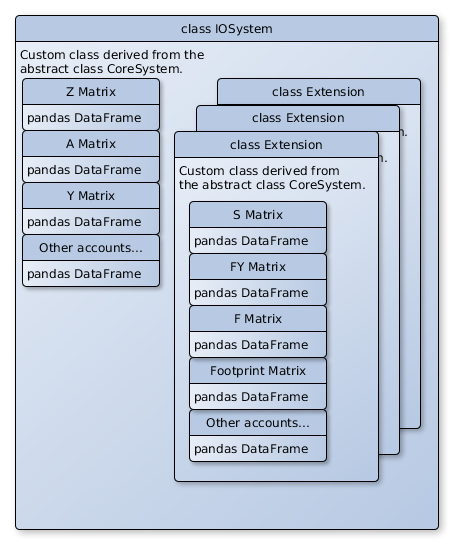
\includegraphics[width=.9\textwidth]{./fig/IOSystem.png}
  \caption{\textbf{Class diagramm of the core Pymrio class.}
  The composite class IOSystem consists of the economic core with the actual data stored in Pandas DataFrames and a variable number of Extension classes. Each Extension consists of multiple Pandas DataFrames. Both, the IOSystem and Extension class are derived from an abstract CoreSystem class implementing the shared functionality of both classes. Class methods are not depicted here.}
  \end{figure}

This architecture described above was implemented in Python 3.6.
The various tables of the MRIO system are stored in Pandas DataFrames \cite{mckinney2010}, therefore building upon a well-tested data-science framework.
As a consequence, besides the specific methods implemented by Pymrio, the full functionality of Pandas and the underlying numpy framework \cite{vanderwalt2011} can be used to modify the MRIO data.

Methods implemented in Pymrio which go beyond basic Pandas functionality are accompanied by a corresponding test harness which ensures the formal correctness of the method.
The full source code is hosted on a public code repository together with an extensive documentation and tutorials \url{https://github.com/konstantinstadler/pymrio}.  
Pymrio is openly available under the GNU General Public License v3.0.

\subsection*{Parsing and Storage}

To date, no standard way of storing MRIO databases has been defined.
For example, the WIOD database \cite{timmer2015} is provided as xlsx tables, whereas Eora \cite{lenzen2013} and EXIOBASE \cite{stadler2018b} use (compressed) csv tables.
For the two latter, however, the approach differs as Eora26 used pure numerical tables with separate files describing the headers, whereas EXIOBASE use csv tables which include the headers.
To ease the use of different MRIO systems, Pymrio include parsers for the different formats.
After parsing a MRIO system, Pymrio stores all data in a consistent way.
For each component (core system and extension) data is stored in a separate folder.
While the storage-format of the actual numerical data can be defined by the user, each storage folder also contains a json file (file\_parameters.json) which contains information about the used format. 
Using the common json file format for storing the file meta data  allows to easily and automatically import the data in other programming environments. 
By default, each tables is stored as a tab-separated text file format, including row and column headers.
The folder with the economic core also contains a file metadata.json which includes information about version, name and system (industry by industry or product by product) as well as a record of modifications to the particular MRIO system (including when it was downloaded, applied aggregations, removal/addition of extensions, etc.). 

\subsection*{Usage}

The following section provides a quick start guide for using Pymrio beginning at the installation followed by a basic input-output calculation example.
For the example here, the WIOD MRIO database \cite{timmer2015} is used. 
However, after downloading and parsing the database the same methods are available for any EE MRIO system.

The code examples here are included as interactive Jupyter notebook  tutorial in the SI.
As the code example here only show the code inputs, refer to the notebook to see the output of a specific command. 
An cloud-based virtual environment with the code example is available at \url{https://mybinder.org/v2/gh/konstantinstadler/pymrio_article/master?filepath=%2Fnotebook%2Fpymrio-tutorial-for-wiod.ipynb}.

Pymrio is a Python \cite{python2018} package, Python version  $\geq$ 3.6 is required.
The Pymrio packages is hosted on PyPI  \cite{pypi2018}  and the Anaconda Cloud \cite{anacondainc.2018}.
Therefore, you can either use
\begin{lstlisting}[language=Bash]
pip install pymrio --upgrade
\end{lstlisting}
or
\begin{lstlisting}[language=Bash]
conda install -c konstantinstadler pymrio
\end{lstlisting}

to install Pymrio and all required packages.

Pymrio can than be used in any Python programming environment.

Throughout the code examples below, it is assumed that Pymrio is imported as follows: 

\begin{lstlisting}
import pymrio
\end{lstlisting}

First, the Pymrio MRIO download function is used to get the WIOD MRIO database with:
\begin{lstlisting}
raw_wiod_path = '/tmp/wiod/raw'
pymrio.download_wiod2013(storage_folder=raw_wiod_path,
                         years=[2008])
\end{lstlisting}

This downloads the 2008 MRIO table from WIOD. Omitting the year parameter would result in a download of all years.
The function returns a Pymrio meta data object, which gives information about the WIOD version, system (in this case industry by industry) and records about from where the data was received (see SI cell 6).

To parse the database into a Pymrio object use:
\begin{lstlisting}
wiod = pymrio.parse_wiod(raw_wiod_path, year=2008)
\end{lstlisting}

The available data can be explored by for example
\begin{lstlisting}
wiod.get_sectors()
wiod.get_regions()
\end{lstlisting}

The transaction matrix can be inspected with
\begin{lstlisting}
wiod.Z
\end{lstlisting}

which returns a panda DataFrame with the recoreded monetary flows.

WIOD includes several extensions, which are stored as sub-objects (see Figure 1) in Pymrio. 
For example, in order to see the AIR emissions provided by WIOD:

\begin{lstlisting}
wiod.AIR.F
\end{lstlisting}

WIOD, however, does neither provide any normalized data (A-matrix, satellite account coefficient data) nor any consumption based accounts (footprints).

In order to calculate them, one could go through all the missing data and compute each account. 
Pymrio provides the required functions, for example to calculate the A-matrix:
\begin{lstlisting}
x = pymrio.calc_x(Z=wiod.Z, Y=wiod.Y)
A = pymrio.calc_A(Z=wiod.Z, x=x)
\end{lstlisting}

Alternativly, Pymrio provides a function which finds all missing accounts and calculates them:
\begin{lstlisting}
wiod.calc_all()
\end{lstlisting}

At this point, a basic EE MRIO analysis is accomplished. For example, the regional consumption based accounts of the AIR emissions are now given by:
\begin{lstlisting}
wiod.AIR.D_cba_reg
\end{lstlisting}

Units are stored separetly in 
\begin{lstlisting}
wiod.AIR.unit
\end{lstlisting}

Pymrio can be linked with the country converter coco \cite{stadler2017} to ease the aggregation of MRIO and results into different classifications.
Using the country converter, WIOD can easily be aggregated into EU and non-EU countries with singling out Germany and the UK by:

\begin{lstlisting}
import country_converter as coco
wiod.aggregate(region_agg = coco.agg_conc(
    original_countries='WIOD',
    aggregates=[{'DEU': 'DEU', 'GBR':'GBR'}, 'EU'],
    missing_countries='Other',
    merge_multiple_string=None))
wiod.rename_regions({'EU':'Rest of EU'}
\end{lstlisting}

To visualize the results for example for CH\textsubscript{4} the matplotlib framework \cite{hunter2007} can be used (Figure 2):
\begin{lstlisting}
import matplotlib.pyplot as plt
with plt.style.context('ggplot'):
    wiod.AIR.plot_account('CH4')
    plt.savefig('airch4.png', dpi=300)
    plt.show()
\end{lstlisting}


  \begin{figure}[h!]
      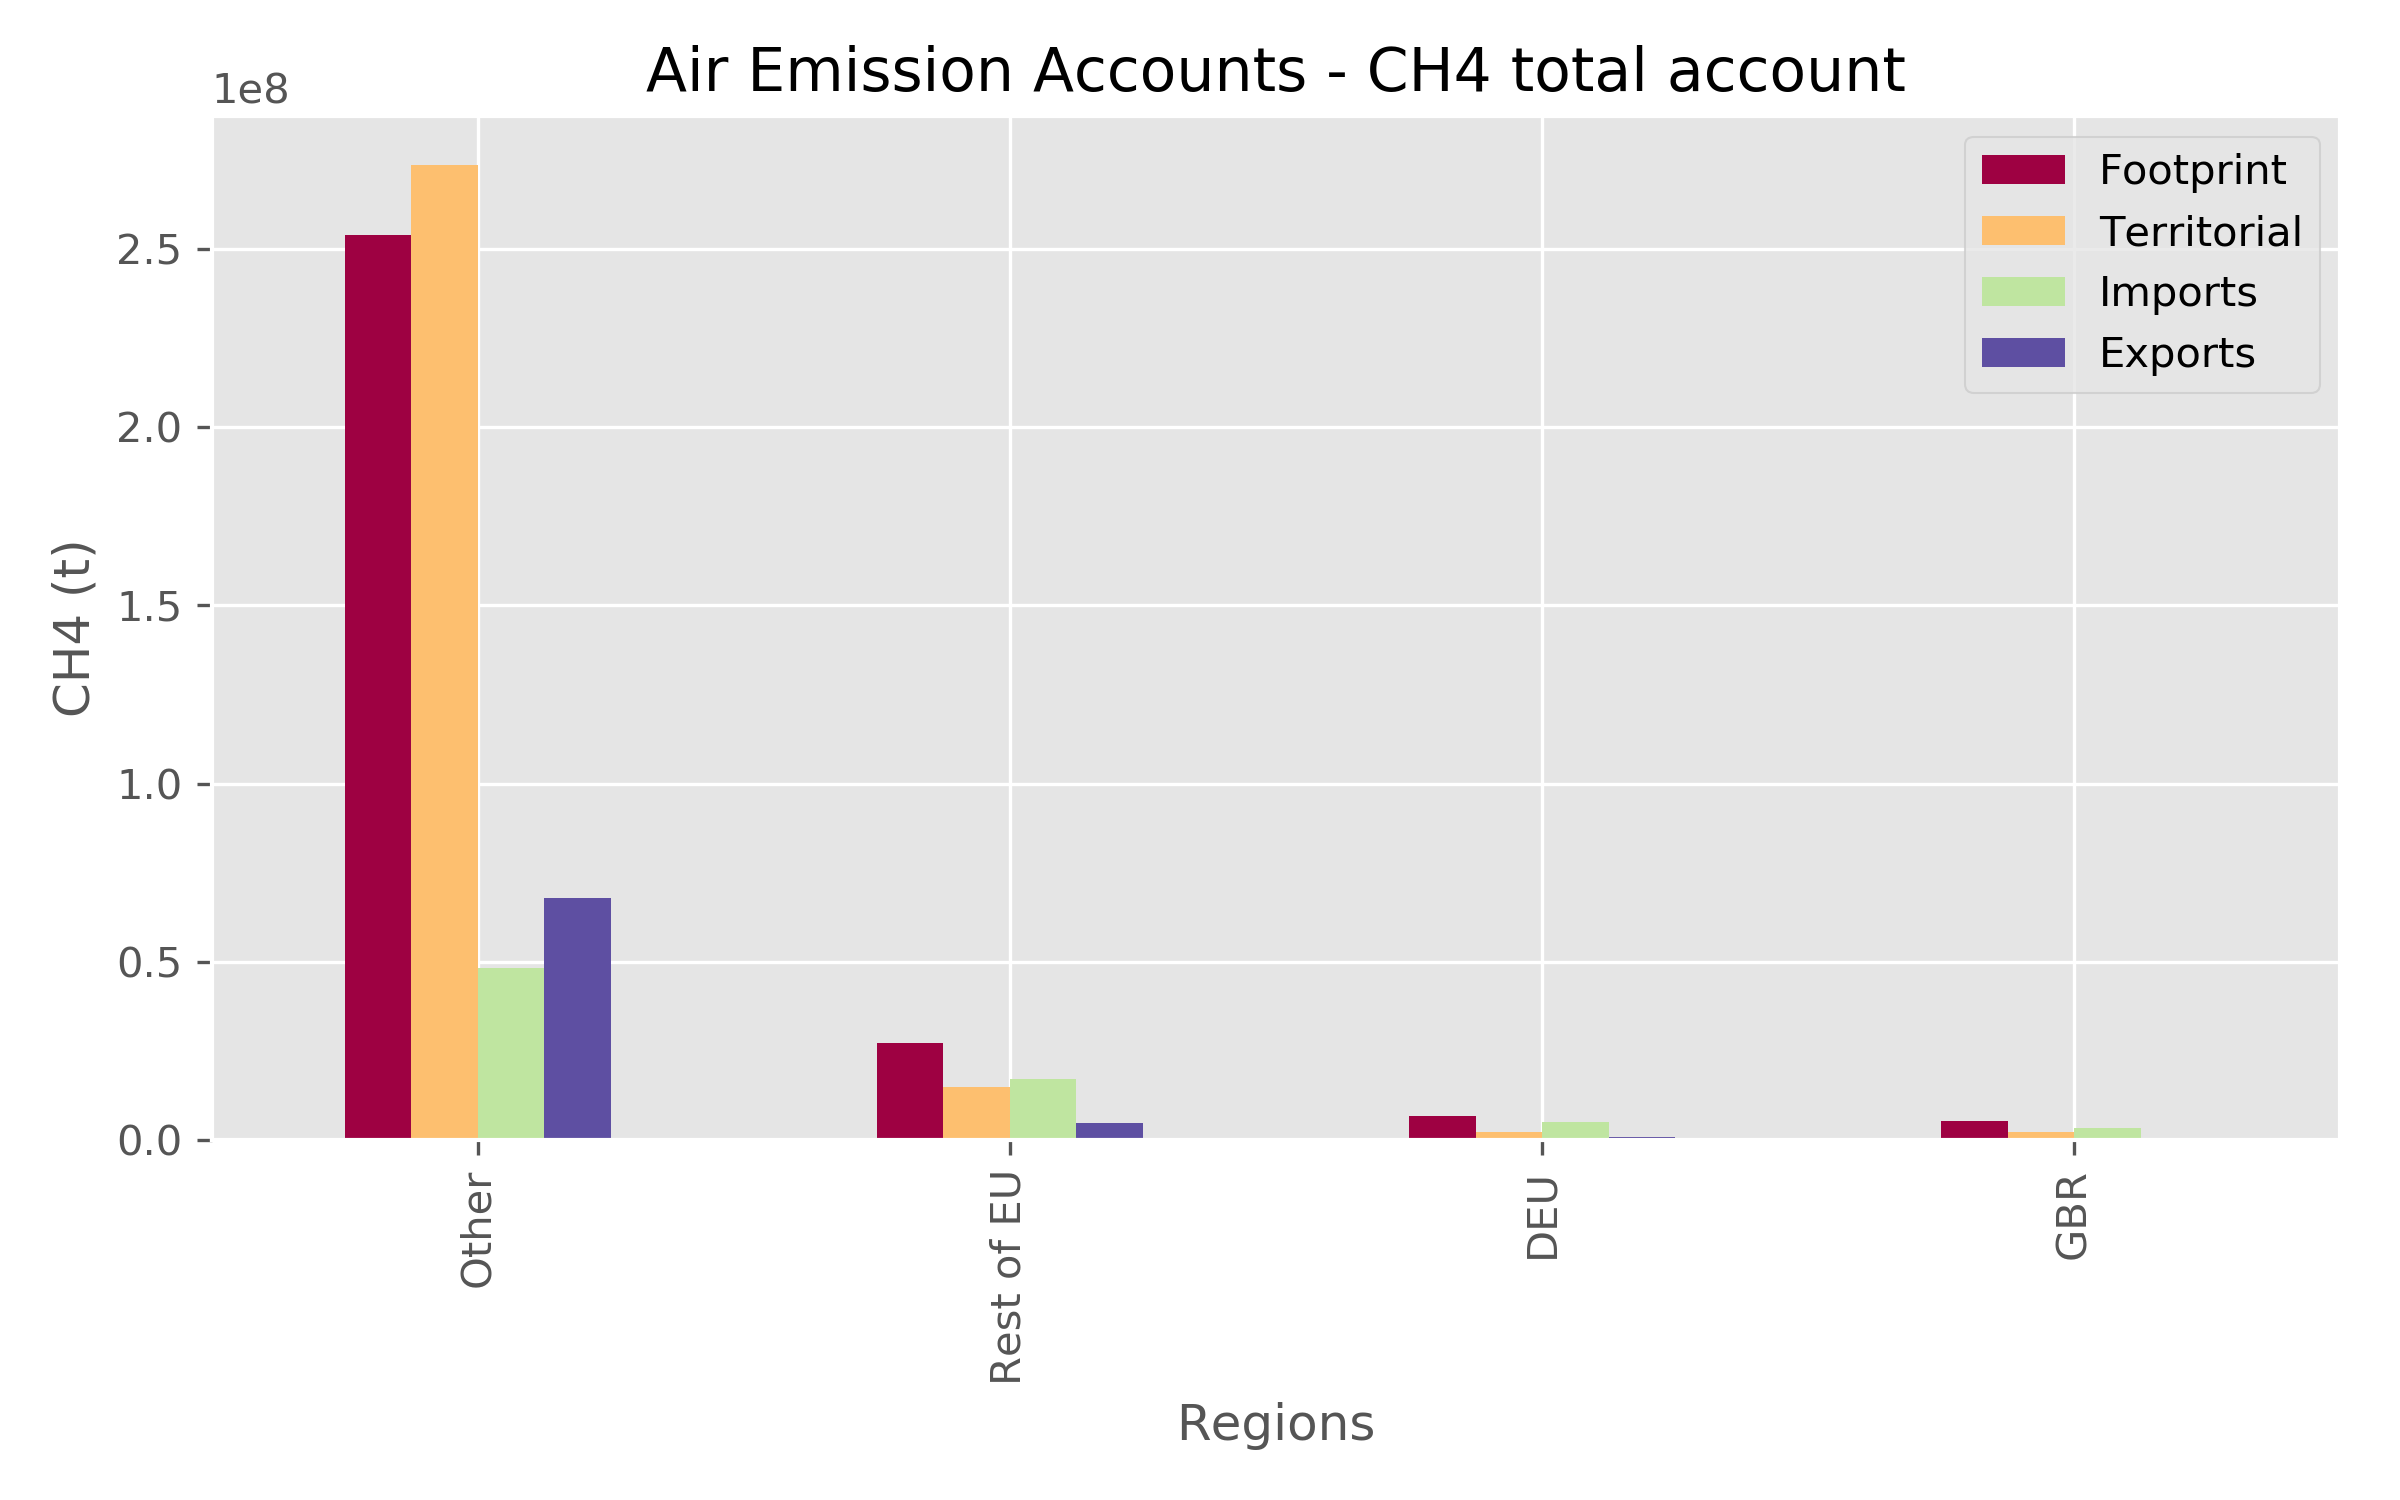
\includegraphics[width=.9\textwidth]{./fig/airch4.png}
      \caption{\textbf{CH\textsubscript{4} emissions of Germany (DEU), the UK (GBR), Rest of the EU and Other countries}
      This figure was produced with Pymrio and matplotlib after aggregating the WIOD countries into the three regions specified above)}
      \end{figure}



To calculate the source (in terms of regions and sectors) of a certain stressor or impact driven by consumption, one needs to diagonalize this stressor/impact. 

This can be done with Pymrio by:
\begin{lstlisting}
diag_CH4 = wiod.AIR.diag_stressor('CH4')
\end{lstlisting}

and be reassigned to the aggregated WIOD system:
\begin{lstlisting}
wiod.CH4_source = diag_CH4
\end{lstlisting}

In the next step the automatic calculation routine of Pymrio is called again to compute the missing accounts in this new extension:

\begin{lstlisting}
wiod.calc_all()
\end{lstlisting}

The diagonalzied CH4 data now shows the source and destination of the specified stressor (CH\textsubscript{4}):
\begin{lstlisting}
wiod.CH4_source.D_cba
\end{lstlisting}

In this square consumption based accounts matrix, every column represents the amount of stressor occurring in each region - sector driven by the consumption stated in the column header. Conversely, each row states where the stressor impacts occurring in the row are distributed to (from where they are driven).

If only one specific aspect of the source is of interest for the analysis, the footprint matrix can easily be aggregated with the standard Pandas {\it groupby} function.
For example, to aggregate to the source and receiving region of the stressor:

\begin{lstlisting}
CH4_source_reg = wiod.CH4_source.D_cba.groupby(
    level='region', axis=0).sum().groupby(
    level='region', axis=1).sum()
\end{lstlisting}

Which can than be visualised using the seaborn heatmap \cite{waskom2017} with (Figure 3):

\begin{lstlisting}
import seaborn as sns
CH4_source_reg.columns.name = 'Receiving region'
CH4_source_reg.index.name = 'Souce region'
sns.heatmap(CH4_source_reg, vmax=5E6, 
            annot=True, cmap='YlOrRd', linewidths=0.1,
            cbar_kws={'label': 'CH4 emissions ({})'.format(
                wiod.CH4_source.unit.unit[0])})
plt.show()
\end{lstlisting}

  \begin{figure}[h!]
      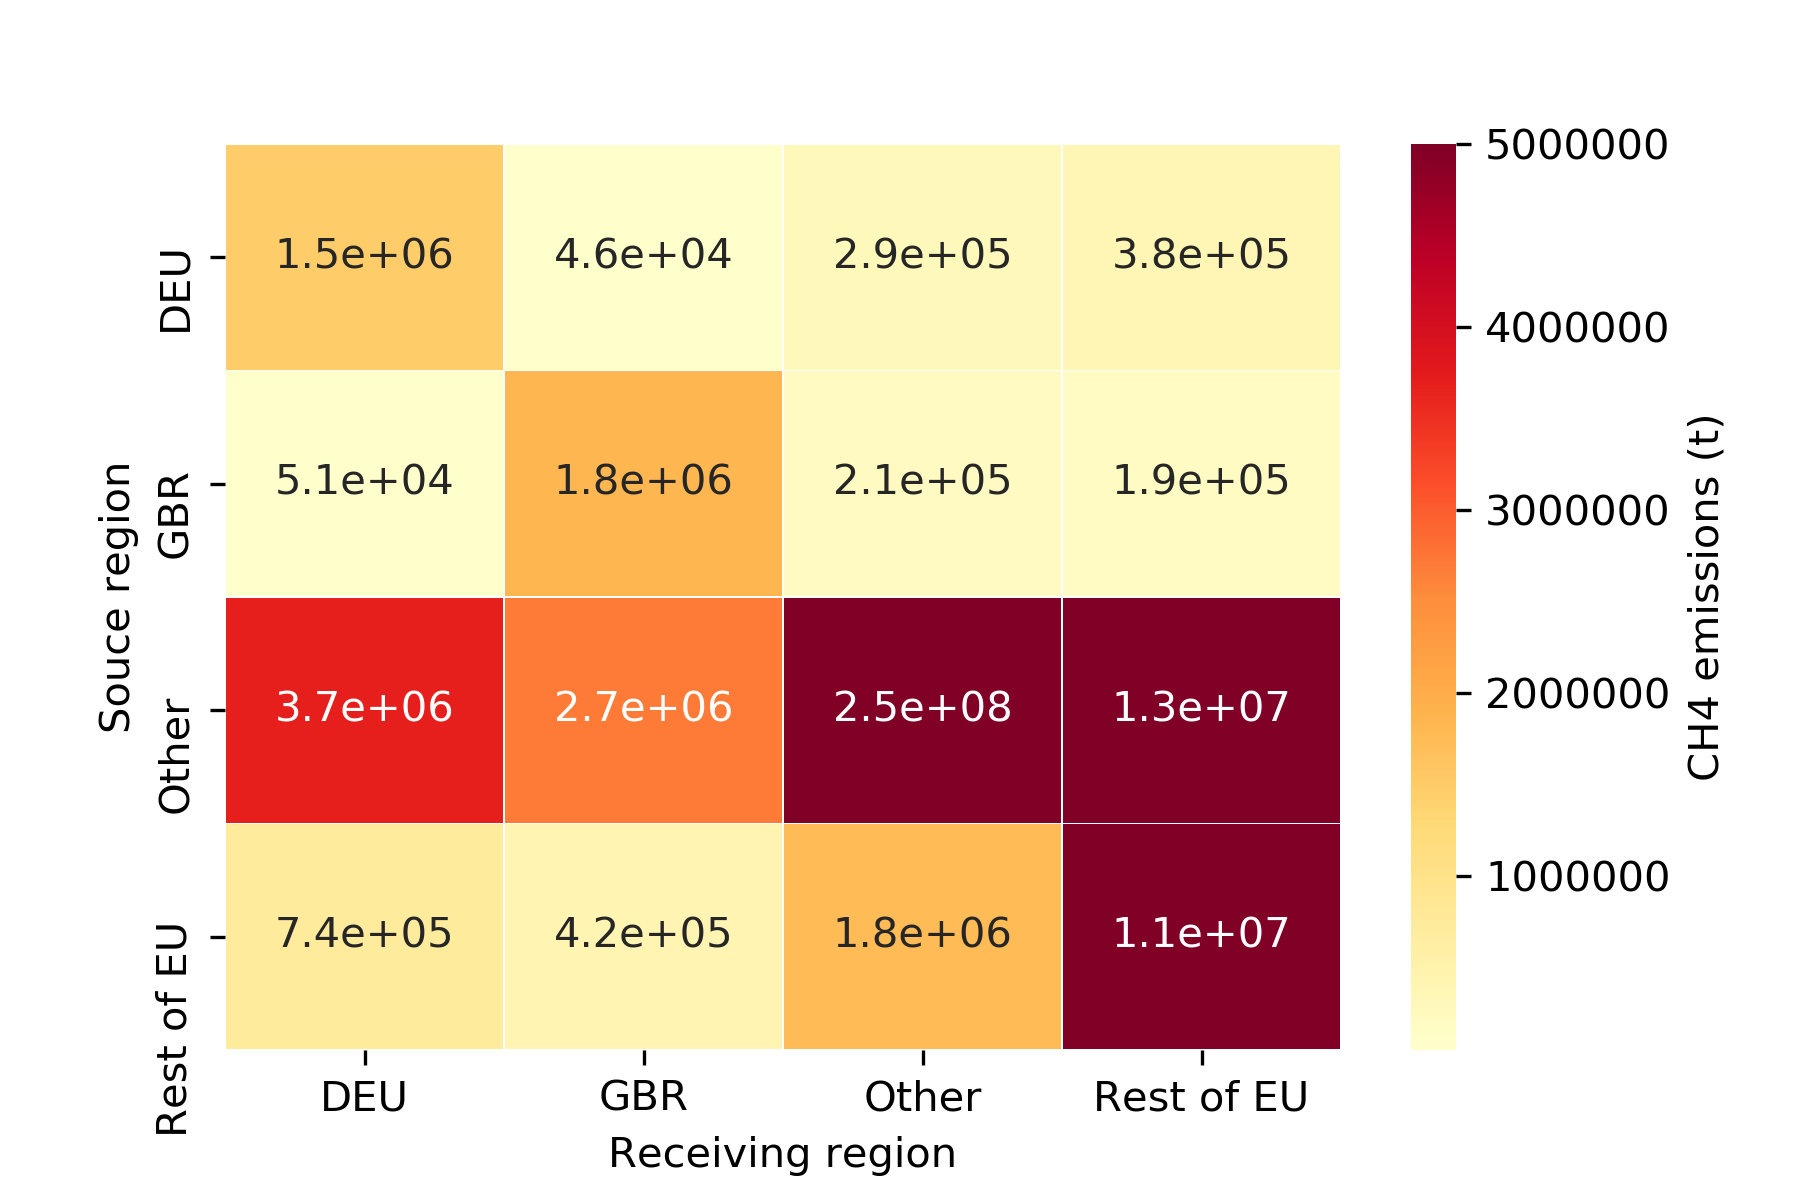
\includegraphics[width=.9\textwidth]{./fig/airch4_source_reg.png}
      \caption{\textbf{CH\textsubscript{4} emissions source and destination}
      A substantial share of CH\textsubscript{4} originating in the Rest of the World region are exported into Germany and the UK.
      This figure was produced with Pymrio and seaborn. }
      \end{figure}


Storing the MRIO database can be done with 

\begin{lstlisting}
storage_path = '/tmp/wiod/aly'
wiod.save_all(storage_path)
\end{lstlisting}

from where it can be received subsequently by:

\begin{lstlisting}
wiod = pymrio.load_all(storage_path)
\end{lstlisting}

The meta attribute of Pymrio mentioned at the beginning kept track of all modifications of the system.
This can be shown with:

\begin{lstlisting}
wiod.meta
\end{lstlisting}

Custom notes can be added to the history with:
\begin{lstlisting}
wiod.meta.note("Custom note")
\end{lstlisting}


The history of the meta data can be filtered for specific entries like:

\begin{lstlisting}
wiod.meta.file_io_history
\end{lstlisting}


This tutorial gave a short overview about the basic functionality of Pymrio. 
For more information about the capabilities of Pymrio check the online documentation at 
\url{http://pymrio.readthedocs.io} 
\cite{stadler2018}



\section*{Quality control}

All basic mathematical functions of Pymrio, as described in the section Mathematical Background above, are unit tested against published results extracted from a classic input-output textbook \cite{miller2009}.
Additional unit tests validate various components of the aggregation, file IO and other utility methods.
Beyond the unit tests, Pymrio includes a small pseudo MRIO system which is used for a full regression test of the package.

All tests are implemented in pytest \cite{krekl2017} and users can verify the correctness of Pymrio, after installing pytest, by

\begin{lstlisting}
py.test -v
\end{lstlisting}

in the root of the local copy of Pymrio.

In addition, Pymrio uses the continous integration platform Travis CI \cite{travis2018} for automatic testing after each change of the code base uploaded to the source repository. 

The Pymrio source code follows the pep8 specifications \cite{rossuml2017}; accordance with this code standard is also tested through Travis CI integration. This implies, that any code contribution to Pymrio must follow the pep8 guidelines.

The Pymrio documentation is build using the Sphinx Python Documentation Generator \cite{brandl2018} and hosted on readthedocs (\url{http://pymrio.readthedocs.io}).

After each change to the master branch, the API references in the documentation are automatically updated based on the description provided in the numpy style docstrings, thus keeping the documentation and code base in sync.
Furthermore, the code examples and tutorials given the in the documentation are implemented as Jupyter notebooks \cite{kluyver2016} and are recalculated for each release, thus also serving as regression tests for the documented Pymrio functionality.

Updated results of the Travis CI tests as well as the Sphinx documentation rebuild are indicated at the beginning of the readme file at the source repository. 

Contributors to the Pymrio code based are advised to adhere to the testing and code standards established for Pymrio. Further details can be found in the Contribution section of the documentation. 

\section*{(2) Availability}
\vspace{0.5cm}
\section*{Operating system}

GNU/Linux, Mac OSX, Windows and any other operating systems running Python with the SciPy stack.

\section*{Programming language}

Pymrio was built in Python 3 and currently (Pymrio version 0.3.6) tested for Python 3.6.


\section*{Additional system requirements}

Pymrio runs on every system capable of running the Python SciPy stack.
The actual memory requirments depend on the MRIO database to be analysed with Pymrio. For example, for EXIOBASE \cite{stadler2018b} a minimum of 8 GB RAM are required. 

\section*{Dependencies}

For the current Pymrio version 0.3.7:

\begin{itemize}
    \item pandas $\ge$ 0.22.0
    \item numpy $\ge$ 0.12.0
    \item matplotlib $\ge$ 2.0.0
    \item requests $\ge$ 2.18
    \item xlrd $\ge$ 1.1.0 
\end{itemize}

The main dependency of Pymrio is Pandas and future versions of Pymrio will follow the developmental changes in Pandas.

The file requirments.txt in the source repository contains an up-to-date list of all requirements.

For development and unit testing, pytest $\ge$ 3.1 \cite{krekl2017} and pytest-pep8 are required.

\section*{Software location:}

{\bf Archive} 

\begin{description}[noitemsep,topsep=0pt]
	\item[Name:] Zenodo
    \item[Persistent identifier:] \url{https://doi.org/10.5281/zenodo.1146054}
	\item[Licence:] GPL v3
	\item[Publisher:]  Konstantin Stadler
    \item[Version published:] 0.3.7 and earlier versions. The DOI above always resolves to the latest version, previous versions can be identified with separate DOIs (see versions sections on the Zenodo repository page). 
    \item[Date published:] 22/10/18 (version 0.3.7)
\end{description}


{\bf Code repository} 

\begin{description}[noitemsep,topsep=0pt]
    \item[Name:] Github (Pymrio is also hosted on pypi and anaconda cloud)
    \item[Persistent identifier:] \url{https://github.com/konstantinstadler/pymrio}
	\item[Licence:] GPL v3
    \item[Date published:] 22/10/18 (version 0.3.7)
\end{description}

{\bf Emulation environment} 

\begin{description}[noitemsep,topsep=0pt]
	\item[Name:] MyBinder Jupyter Notebook of the tutorial included above
    \item[Persistent identifier:] \url{https://mybinder.org/v2/gh/konstantinstadler/pymrio_article/master?filepath=%2Fnotebook%2Fpymrio-tutorial-for-wiod.ipynb}
        \item[Licence:] CC BY 4.0 (TODO - identifier in Binder Notebook) 
	\item[Date published:] 18/01/18
\end{description}

\section*{Language}

English

\section*{(3) Reuse potential}

Pymrio contains functionality aimed at professional MRIO analysts and sustainability scientist, but might be useful to anyone doing environmental and/or economic analysis. 
As such, Pymrio is one key component in the Industrial Ecology analysis software framework \cite{pauliuk2015}.
With the other components it shares the ambition to improve usability, interoperability, and collaboration between Industrial Ecology and sustainability research Python packages.
The main motivation for starting the project was to enable a common interface for handling different MRIO databases, but through the years the scope extended to include visualization, reporting and data provenance tracking capabilities.
Future development plans include further visualization possibilities, parser for additional MRIO models and extended analysis capabilities like structural decomposition and structural path analysis.
Being an open source project, this includes an invitation to fellow researchers to join these coding efforts.

The primary communication channel for Pymrio is the GitHub source repository, in particular the Issue Tracker there. 
I strongly encouraged to not only use the Issue Tracker for bug reporting but for all questions, comments, and suggestions regarding the project.
Pymrio follows an "issue driven" development style. This means that the first step for any modifications or enhancements to Pymrio are to file an issue describing the planned changes.
This allows us to discuss changes before the actual programming and gives us the chance to identify synergies across ongoing efforts and avoid potential double work. 
Finished modification should than be submited as pull request. Further information about open points and code style can be found in the contributing.rst file at the source repository.

\section*{Acknowledgements}
Special thanks to 
Guillaume Majeau-Bettez (Polytechnique Montréal / Norwegian University of Science and Technology), 
Radek Lonka (Norwegian University of Science and Technology),
Richard Wood (Norwegian University of Science and Technology) and
Stefan Pauliuk (University of Freiburg) 
for discussing ideas and the scope of Pymrio as well as implementation details.
Much oblidged also to all people already using Pymrio and providing feedback and improvement suggestions. 


\section*{Funding statement}

Parts of the development of Pymrio was funded by the European Commission under the DESIRE Project (grant no.: 308552).

\section*{Competing interests}

The authors declare that they have no competing interests.



\bibliographystyle{bmc-mathphys}
\bibliography{bibpymrio}  

\vspace{2cm}

\rule{\textwidth}{1pt}

{ \bf Copyright Notice} \\
Authors who publish with this journal agree to the following terms: \\

Authors retain copyright and grant the journal right of first publication with the work simultaneously licensed under a  \href{http://creativecommons.org/licenses/by/3.0/}{Creative Commons Attribution License} that allows others to share the work with an acknowledgement of the work's authorship and initial publication in this journal. \\

Authors are able to enter into separate, additional contractual arrangements for the non-exclusive distribution of the journal's published version of the work (e.g., post it to an institutional repository or publish it in a book), with an acknowledgement of its initial publication in this journal. \\

By submitting this paper you agree to the terms of this Copyright Notice, which will apply to this submission if and when it is published by this journal.

\end{document}
